\documentclass[oneside,a4paper]{report}
\usepackage{color}
\usepackage{longtable}
\usepackage{titlesec}
\usepackage[hidelinks]{hyperref}
\usepackage{ulem}
\usepackage{float}
\usepackage{graphicx}
\usepackage{fancyhdr}
\usepackage{rotating}
\usepackage[T1]{fontenc}
\usepackage[headheight=25pt,margin=0.7in,top=1.5in,bottom=1in,right=1in,left=1in]{geometry}

\hypersetup{colorlinks=true,linktoc=none,citecolor=black,urlcolor=blue}
\hypersetup{linktocpage=false,linkcolor=black}

\pagestyle{fancy}
\fancyhead[R]{
\includegraphics[width=2cm]{./latex/resources/kitlogo.png}}
\fancyhead[L]{\leftmark}

\fancypagestyle{plain}{
        \rhead{
\includegraphics[width=2cm]{./latex/resources/kitlogo.png}}
        \lhead{\leftmark}
}


\renewcommand{\arraystretch}{2}

\titleformat{\chapter}[hang]
 {\normalfont\bfseries\LARGE}{\thechapter. }{0pt}{\LARGE}
\titleformat{\section}[hang]
 {\normalfont\bfseries\Large}{\thesection. }{0pt}{\Large}
\titleformat{\paragraph}[hang]
 {\normalfont\bfseries\normalsize}{}{}{}

\titlespacing*{\chapter}{0pt}{-20pt}{10pt}

\begin{document}
  \begin{titlepage}
	\centering
	{\scshape\LARGE Karlsruhe Institute of Technology \par}
	\vspace{1cm}
	{\scshape\Large Software Engineering Practice\par}
	\vspace{0.5cm}
	{\scshape\Large WINTER TERM 2015/2016\par}
	\vspace{1.5cm}
	{\Huge\bfseries rootJS - module guide\par}
	\vspace{0.25cm}
	{\Large\bfseries Node.js bindings for ROOT 6\par}
	\vspace{2cm}
	{\Large\itshape Jonas Schwabe\par}
	{\Large\itshape Theo Beffart\par}
	{\Large\itshape Sachin Rajgopal\par}
	{\Large\itshape Christoph Wolff\par}
	{\Large\itshape Christoph Haas\par}

	{\Large\itshape Maximilian Fr\"uh\par}
	\vfill
	supervised by\par
	Dr.~Marek \textsc{Szuba}

	\vfill

	% Bottom of the page
	{\large \date{99.99.9999}\par}
\end{titlepage}

  \tableofcontents
  \clearpage
\chapter{Introduction}
\section{About this document}
This document describes the structure of RootJS, it will be used as a blueprint in the implementation phase.

The document contains descriptions to all public methods, so that the implementation can be split up, it contains all classes that need to be implemented, descriptions to all public methods and, listed in the UML diagram in the appendix, some private functions and properties that might be handy during implementation.

\section{Overview}
When using node moldues to extend the basic node api, one uses the \textit{require} statement, providing the name of the module.
require returns a JavaScript object wich is called exports, containing everyting the node modules decides to include.

In our case require will run the \textit{initilize} method which will crawl trough ROOT to find all gloablly accessible variables, functions and classes.

For all these items a property or function is being added to the exports object.
These properties are bound to a callback function which is equipped with meta data, refereing to the property or function in ROOT.
With this information the callback function is able to call the actual ROOT functionality.

To send the results to node we need to convert the resulting objects or values.
In order to convert the data we will use proxys for the different datatypes that will be returned by a factory.\\

The factory will use the datatype to select a matching Proxy implementation, when dealing with non scalar data, the factory will run through all methods and properties and use the Factory recursively.\\

Even though node programs are mainly used as server applications it can still handle graphical user interfaces.
Graphical user interfaces need to refresh frequently in order to be responsive, as JavaScript only runs one thread at a time, the gui refresh needs to run on the same thread as the rest of the application. Graphical user interfaces are therefor supported as well.

This is handled in the \textit{NodeApplication} class, further we will set the application name and a callback function for messages generated by root here.

\chapter{CallbackHandler}
The CallbackHandler class gets invoked whenever an encapsulated ROOT function or object is accessed.
\section{ctorCallback}
\begin{longtable}{p{3cm} @{\hskip 1cm} p{12cm}}
 \hline
\textit{Name} & \texttt{CallbackHandler::ctorCallback(args: FunctionCallbackInfo<Value>)}\\
\hline
 \textit{Visibility} & public\\
\hline
\textit{Parameters} & \textit{args: FunctionCallbackInfo<Value>} information about the context\\
\hline
\textit{Return value} & \textbf{none}\\
  \hline
 \textit{Behavior} & Gets invoked whenever a non static constructor function of an encapsulated ROOT class was called.\\
\hline
\end{longtable} \pagebreak
 \section{staticCtorCallback}
\begin{longtable}{p{3cm} @{\hskip 1cm} p{12cm}}
 \hline
\textit{Name} & \texttt{CallbackHandler::staticCtorCallback(args: FunctionCallbackInfo<Value>)}\\
\hline
 \textit{Visibility} & public\\
\hline
\textit{Parameters} & \textit{args: FunctionCallbackInfo<Value>}\\
\hline
\textit{Return value} & \textbf{none}\\
  \hline
 \textit{Behavior} & Gets invoked whenever a static constructor of an encapsulated ROOT class was called.\\
\hline
\end{longtable} \pagebreak
 \section{memberGetterCallback}
\begin{longtable}{p{3cm} @{\hskip 1cm} p{12cm}}
 \hline
\textit{Name} & \texttt{CallbackHandler::memberGetterCallback(property: Local<String>, info: PropertyCallbackInfo<Value>)}\\
\hline
 \textit{Visibility} & public\\
\hline
\textit{Parameters} & \textit{property: Local<String>, info: PropertyCallbackInfo<Value>}\\
\hline
\textit{Return value} & \textbf{none}\\
  \hline
 \textit{Behavior} & Gets invoked whenever an encapsulated (class) member was requested.\\
\hline
\end{longtable} \pagebreak
 \section{memberSetterCallback}
\begin{longtable}{p{3cm} @{\hskip 1cm} p{12cm}}
 \hline
\textit{Name} & \texttt{CallbackHandler::memberSetterCallback(property: Local<String>, value: Local<Value>, info: PropertyCallbackInfo<Value>)}\\
\hline
 \textit{Visibility} & public\\
\hline
\textit{Parameters} & \textit{property: Local<String>, value: Local<Value>, info: PropertyCallbackInfo<Value>}\\
\hline
\textit{Return value} & \textbf{none}\\
  \hline
 \textit{Behavior} & Gets invoked whenever an encapsulated (class) member is attempted to be set.\\
\hline
\end{longtable} \pagebreak
 \section{memberFunctionCallback}
\begin{longtable}{p{3cm} @{\hskip 1cm} p{12cm}}
 \hline
\textit{Name} & \texttt{CallbackHandler::memberFunctionCallback(args: FunctionCallbackInfo<Value>)}\\
\hline
 \textit{Visibility} & public\\
\hline
\textit{Parameters} & \textit{args: FunctionCallbackInfo<Value>}\\
\hline
\textit{Return value} & \textbf{none}\\
  \hline
 \textit{Behavior} & Gets invoked whenever an non-static (class) function was called.\\
\hline
\end{longtable} \pagebreak
 \section{staticGetterCallback}
\begin{longtable}{p{3cm} @{\hskip 1cm} p{12cm}}
 \hline
\textit{Name} & \texttt{CallbackHandler::staticGetterCallback(property: Local<String>, info: PropertyCallbackInfo<Value>)}\\
\hline
 \textit{Visibility} & public\\
\hline
\textit{Parameters} & \textit{property: Local<String>, info: PropertyCallbackInfo<Value>}\\
\hline
\textit{Return value} & \textbf{none}\\
  \hline
 \textit{Behavior} &  Gets invoked whenever an encapsulated static object was requested.\\
\hline
\end{longtable} \pagebreak
 \section{staticSetterCallback}
\begin{longtable}{p{3cm} @{\hskip 1cm} p{12cm}}
 \hline
\textit{Name} & \texttt{CallbackHandler::staticSetterCallback(property: Local<String>, value: Local<Value>, info: PropertyCallbackInfo<Value>)}\\
\hline
 \textit{Visibility} & public\\
\hline
\textit{Parameters} & \textit{property: Local<String>, value: Local<Value>, info: PropertyCallbackInfo<Value>}\\
\hline
\textit{Return value} & \textbf{none}\\
  \hline
 \textit{Behavior} & Gets invoked whenever an encapsulated static object is attempted to be set.\\
\hline
\end{longtable} \pagebreak
 \section{staticFunctionCallback}
\begin{longtable}{p{3cm} @{\hskip 1cm} p{12cm}}
 \hline
\textit{Name} & \texttt{CallbackHandler::staticFunctionCallback(args: FunctionCallbackInfo<Value>)}\\
\hline
 \textit{Visibility} & public\\
\hline
\textit{Parameters} & \textit{args: FunctionCallbackInfo<Value>}\\
\hline
\textit{Return value} & \textbf{none}\\
  \hline
 \textit{Behavior} & Gets invoked whenever a static function was called.\\
\hline
\end{longtable} \pagebreak

\chapter{NodeHandler}
describe class NodeHandler here
\section{getExports}
\begin{longtable}{p{3cm} @{\hskip 1cm} p{12cm}}
 \hline
\textit{Name} & \texttt{NodeHandler::getExports()}\\
\hline
 \textit{Visibility} & public\\
\hline
\textit{Parameters} & \textit{none}\\
\hline
\textit{Return value} & \textbf{ Local<Object>} describe return value\\
  \hline
 \textit{behavior} & describe beahviour \\
\hline
\end{longtable} \pagebreak
 
\chapter{NodeApplication}
describe class NodeApplication here
\section{NodeApplication}
\begin{longtable}{p{3cm} @{\hskip 1cm} p{12cm}}
 \hline
\textit{Name} & \texttt{NodeApplication::NodeApplication(acn: char*, argc: int*, argv: char**)}\\
\hline
 \textit{Visibility} & public\\
\hline
\textit{Parameters} & \textit{acn: char*, argc: int*, argv: char**}\\
\hline
\textit{Return value} & \textbf{ <<constructor>>} describe return value\\
  \hline
 \textit{Behavior} & describe beahviour \\
\hline
\end{longtable} \pagebreak
 
\chapter{TemplateFactory}
Creates Javascript function templates from a given ROOT class using \textit{TClassRef}. Methods and static members are set during creation through the use of ROOT reflections and the proxy factories.

\section{createTemplate}
\begin{longtable}{p{3cm} @{\hskip 1cm} p{12cm}}
 \hline
\textit{Name} & \texttt{TemplateFactory::createTemplate(clazz: TClassRef)}\\
\hline
 \textit{Visibility} & public\\
\hline
\textit{Parameters} & \textit{clazz: TClassRef} the class for which a template is to be created \\
\hline
\textit{Return value} & \textbf{Local<FunctionTemplate>} the created template\\
  \hline
 \textit{Behavior} & Gets the class from TClassRef and creates a new function template.
			Then it iterates over all static members of the class and sets the
			corresponding members of the template to respective proxy objects.
			It then iterates through the functions and also sets them.
			For further reference consider the following sequence diagram.\\
\hline
\end{longtable} \pagebreak

\begin{figure}[htb]
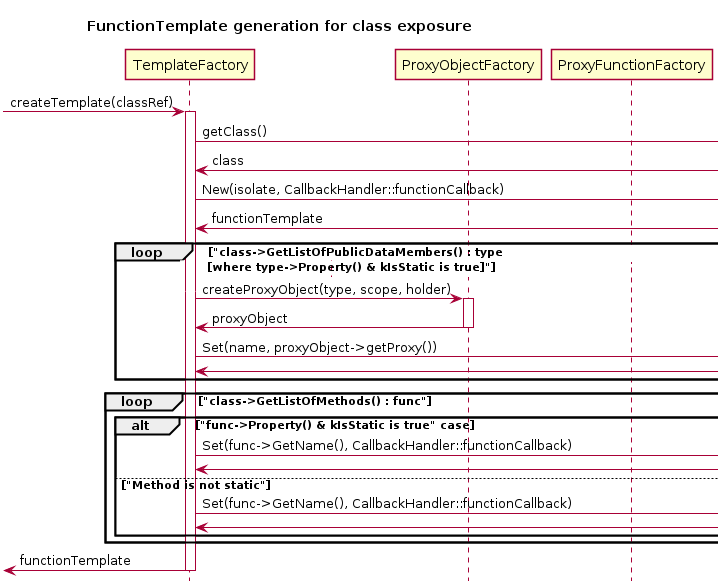
\includegraphics[width=16cm]{./latex/resources/functionTemplateGenerateCrop.png}
	\caption{function template creation (full diagram in appendix)}
\end{figure}

\chapter{Proxy}
The \textit{Proxy} class is an abstract class which acts as an intermediary between Node.js and ROOT. Both the \textit{ObjectProxy} and \textit{FunctionProxy} inherit the \textit{Proxy} class. Both of them require the object's or function's \textit{void*} address to access the original ROOT object. The \textit{TObject} type is more accurately specified in each class which inherits \textit{Proxy}. The \textit{TClassRef} scope is used to access \textit{TClass} and the necessary information about the class. The \textit{Proxy} class holds the data, which both \textit{ObjectProxy} and \textit{FunctionProxy} require. The \textit{Proxy} class uses the Proxy design pattern.
\section{Proxy}
\begin{longtable}{p{3cm} @{\hskip 1cm} p{12cm}}
 \hline
\textit{Name} & \texttt{Proxy::Proxy(address: void*, type: TObject, scope: TClassRef)}\\
\hline
 \textit{Visibility} & protected\\
\hline
\textit{Parameters} & \textit{address: void*} The memory address of the ROOT object \\
& \textit{type: TObject}  The type of Object will be specified in the subclasses \\
& \textit{scope: TClassRef} The reference of the TClass so that it can be accessed  \\
\hline
\textit{Return value} & \textbf{<<constructor>>} Returns a Proxy with the given parameters as a variables \\
  \hline
 \textit{Behavior} & The Proxy constructor will be inherited by both ObjectProxy and FunctionProxy.
 The created Proxy will have the parameters as variables. \\
\hline
\end{longtable} \pagebreak
 \section{setAddress}
\begin{longtable}{p{3cm} @{\hskip 1cm} p{12cm}}
 \hline
\textit{Name} & \texttt{Proxy::setAddress(address: void*)}\\
\hline
 \textit{Visibility} & public\\
\hline
\textit{Parameters} & \textit{address: void*} The address to which the proxied ROOT object should be set to \\
\hline
\textit{Return value} & \textbf{none}\\
  \hline
 \textit{Behavior} & Sets the address of the proxied ROOT object. \\
\hline
\end{longtable} \pagebreak
 \section{getAddress}
\begin{longtable}{p{3cm} @{\hskip 1cm} p{12cm}}
 \hline
\textit{Name} & \texttt{Proxy::getAddress()}\\
\hline
 \textit{Visibility} & public\\
\hline
\textit{Parameters} & \textit{none}\\
\hline
\textit{Return value} & \textbf{void*} The current address of the proxied ROOT object \\
  \hline
 \textit{Behavior} & Gets the current address of the proxied ROOT object. \\
\hline
\end{longtable} \pagebreak
 \section{getType}
\begin{longtable}{p{3cm} @{\hskip 1cm} p{12cm}}
 \hline
\textit{Name} & \texttt{Proxy::getType()}\\
\hline
 \textit{Visibility} & public\\
\hline
\textit{Parameters} & \textit{none}\\
\hline
\textit{Return value} & \textbf{TObject} The current type of the proxied ROOT object \\
  \hline
 \textit{Behavior} & Gets the current type of the proxied ROOT object. \\
\hline
\end{longtable} \pagebreak
 \section{getScope}
\begin{longtable}{p{3cm} @{\hskip 1cm} p{12cm}}
 \hline
\textit{Name} & \texttt{Proxy::getScope()}\\
\hline
 \textit{Visibility} & public\\
\hline
\textit{Parameters} & \textit{none}\\
\hline
\textit{Return value} & \textbf{TClassRef} The current scope of the proxied ROOT object \\
  \hline
 \textit{Behavior} & Gets the current scope of the proxied ROOT object. \\
\hline
\end{longtable} \pagebreak
 \section{isGlobal}
\begin{longtable}{p{3cm} @{\hskip 1cm} p{12cm}}
 \hline
\textit{Name} & \texttt{Proxy::isGlobal()}\\
\hline
 \textit{Visibility} & public\\
\hline
\textit{Parameters} & \textit{none}\\
\hline
\textit{Return value} & \textbf{bool} True if the Proxy is global \\
  \hline
 \textit{Behavior} & Checks if the Proxy is global and hence visible throughout the program. \\
\hline
\end{longtable} \pagebreak
 \section{isTemplate}
\begin{longtable}{p{3cm} @{\hskip 1cm} p{12cm}}
 \hline
\textit{Name} & \texttt{Proxy::isTemplate()}\\
\hline
 \textit{Visibility} & public\\
\hline
\textit{Parameters} & \textit{none}\\
\hline
\textit{Return value} & \textbf{bool} True if the Proxy is a template \\
  \hline
 \textit{Behavior} & Checks if the Proxy is a template, which allows using generic types. \\
\hline
\end{longtable} \pagebreak
 \section{isConst}
\begin{longtable}{p{3cm} @{\hskip 1cm} p{12cm}}
 \hline
\textit{Name} & \texttt{Proxy::isConst()}\\
\hline
 \textit{Visibility} & public\\
\hline
\textit{Parameters} & \textit{none}\\
\hline
\textit{Return value} & \textbf{bool} True if the Proxy is a constant \\
  \hline
 \textit{Behavior} & Checks if the Proxy is a constant. \\
\hline
\end{longtable} \pagebreak
 \section{isStatic}
\begin{longtable}{p{3cm} @{\hskip 1cm} p{12cm}}
 \hline
\textit{Name} & \texttt{Proxy::isStatic()}\\
\hline
 \textit{Visibility} & public\\
\hline
\textit{Parameters} & \textit{none}\\
\hline
\textit{Return value} & \textbf{bool} True if the Proxy is static \\
  \hline
 \textit{Behavior} & Checks if the Proxy is static. \\
\hline
\end{longtable} \pagebreak

\chapter{FunctionProxyFactory}
The \textit{FunctionProxyFactory} creates \textit{FunctionProxy} instances with \textit{TFunction} function and \textit{TClassRef} scope. It encapsulates ROOT functions recursively for use in Javascript. 
\section{createFunctionProxy}
\begin{longtable}{p{3cm} @{\hskip 1cm} p{12cm}}
 \hline
\textit{Name} & \texttt{FunctionProxyFactory::createFunctionProxy(function: TFunction, scope: TClassRef)}\\
\hline
 \textit{Visibility} & public\\
\hline
\textit{Parameters} & \textit{function: TFunction, scope: TClassRef}\\
\hline
\textit{Return value} & \textbf{ ProxyFunciton} describe return value\\
  \hline
 \textit{Behavior} & describe beahviour \\
\hline
\end{longtable} \pagebreak
 \section{fromArgs}
\begin{longtable}{p{3cm} @{\hskip 1cm} p{12cm}}
 \hline
\textit{Name} & \texttt{FunctionProxyFactory::fromArgs(name: string, scope: TClassRef, args: FunctionCallbackInfo)}\\
\hline
 \textit{Visibility} & public\\
\hline
\textit{Parameters} & \textit{name: string, scope: TClassRef, args: FunctionCallbackInfo}\\
\hline
\textit{Return value} & \textbf{ FunctionProxy} describe return value\\
  \hline
 \textit{Behavior} & describe beahviour \\
\hline
\end{longtable} \pagebreak
 
\chapter{FunctionProxy}
In order to make ROOT callable functions and methods dynamically accessible within the Node.js application, they need to be proxied. The \textit{FunctionProxy} provides such functionality, as well as acting as a static cache for commonly used \textit{FunctionProxy} objects.\\
\\
A \textit{FunctionProxy} instance holds a pointer to the callable function's and method's location in main memory, and reflection data, such as the callable's signature. It also provides functionality to validate parameters and encapsulate them within \textit{ObjectProxy} instances. The \textit{FunctionProxy::call} method can then be used to execute the callable using the \textit{ObjectProxy} instances as parameters. The return value is again encapsulated within an \textit{ObjectProxy} and returned to the caller.\\
As JavaScript does not support overloading, but C++ does, the \textit{FunctionProxy} can be used to statically get all methods with a specified name. The \textit{FunctionProxy} also maintains a static cache which maps functions and methods to their memory location. This is useful for creating new \textit{FunctionProxy instances}.\\

\section{getCallFunc}
\begin{longtable}{p{3cm} @{\hskip 1cm} p{12cm}}
	\hline

	\textit{Name} & \texttt{FunctionProxy::getCallFunc(method: TFunction*)}\\
	\hline

	\textit{Visibility} & public\\
	\hline

	\textit{Parameters} &  \textit{method: TFunction*}: pointer to the ROOT function for which a proxy 
							is to be created\\
	\hline

	\textit{Return value} & \textbf{CallFunc*} a pointer to the CallFunc object provided by cling\\
	\hline

	\textit{Behavior} & Gets a pointer to a \textit{CallFunc} object, which encapsulates the provided ROOT function in memory.\\
	\hline

\end{longtable} 

\section{getMethodsFromName}
\begin{longtable}{p{3cm} @{\hskip 1cm} p{12cm}}
	\hline

	\textit{Name} & \texttt{FunctionProxy::getMethodsFromName(scope: TClassRef, name: string)}\\
	\hline

	\textit{Visibility} & public\\
	\hline

	\textit{Parameters} & \textit{scope: TClassRef} reference to the class which is checked for methods with the specified name\\
		& \textit{name: string} name of the overloaded methods which shall be returned\\
	\hline

	\textit{Return value} & \textbf{vector<TFunction*>} methods that match the specified name\\
	\hline

	\textit{Behavior} & Gets a reference to a class and a method name string. It returns all methods of the class with the specified name. This is needed since JavaScript does not support method overloading.\\
	\hline

\end{longtable}
\pagebreak

\section{FunctionProxy}
\begin{longtable}{p{3cm} @{\hskip 1cm} p{12cm}}
	\hline

	\textit{Name} & \texttt{FunctionProxy::FunctionProxy(address: void*, function: TFunction, scope: TClassRef)}\\
	\hline

	\textit{Visibility} & public\\
	\hline

	\textit{Parameters} & \textit{address: void*} memory address of the proxied function\\
		& \textit{function: TFunction} the function's reflection object\\
		& \textit{scope: TClassRef} the class that the function belongs to\\
	\hline

	\textit{Return value} & \textbf{<<constructor>>} the created \textit{FunctionProxy}\\
	\hline

	\textit{Behavior} & Creates the \textit{FunctionProxy}.\\
	\hline

\end{longtable}


\section{getType}
\begin{longtable}{p{3cm} @{\hskip 1cm} p{12cm}}
	\hline

	\textit{Name} & \texttt{FunctionProxy::getType()}\\
	\hline

	\textit{Visibility} & public\\
	\hline

	\textit{Parameters} & \textit{none}\\
	\hline

	\textit{Return value} & \textbf{TFunction} the \textit{TFunction} object that contains the function's reflection data\\
	\hline

	\textit{Behavior} & Returns the wrapped function's \textit{TFunction} object. It contains the meta data of its corresponding function.\\
	\hline

\end{longtable}


\section{validateArgs}
\begin{longtable}{p{3cm} @{\hskip 1cm} p{12cm}}
	\hline

	\textit{Name} & \texttt{FunctionProxy::validateArgs(args: FunctionCallbackInfo)}\\
	\hline

	\textit{Visibility} & public\\
	\hline

	\textit{Parameters} & \textit{args: FunctionCallbackInfo} information about the context of the call, including the number and values of arguments\\
	\hline

	\textit{Return value} & \textbf{ObjectProxy[]} array of the arguments as proxies\\
	\hline

	\textit{Behavior} & Checks whether the function is being called with the proper arguments and wraps them in proxies so they can be used by the call method.\\
	\hline

\end{longtable}
\pagebreak

\section{call}
\begin{longtable}{p{3cm} @{\hskip 1cm} p{12cm}}
	\hline

	\textit{Name} & \texttt{FunctionProxy::call(args: ObjectProxy[])}\\
	\hline

	\textit{Visibility} & public\\
	\hline

	\textit{Parameters} & \textit{args: ObjectProxy[]} proxies containing arguments for the method\\
	\hline

	\textit{Return value} & \textbf{ObjectProxy} proxy for the object returned by the called method\\
	\hline

	\textit{Behavior} & Calls the actual method in memory using Cling. The argument object proxies' contents are read and given to the called method.\\
	\hline

\end{longtable}
\pagebreak

\chapter{ObjectProxyFactory}
The \textit{ObjectProxyFactory} creates \textit{ObjectProxy} instances with \textit{TDataMember} type, \textit{TClassRef} scope and \textit{ObjectProxy} holder. It encapsulates ROOT objects recursively for use in Javascript.\\

To handle circular references we need to maintain a cache of already generated \textit{ProxyObject}s, which will only be valid during object conversion. Whenever an object is cached it will be used instead of creating a new one.
\begin{figure}[H]
	\centering
	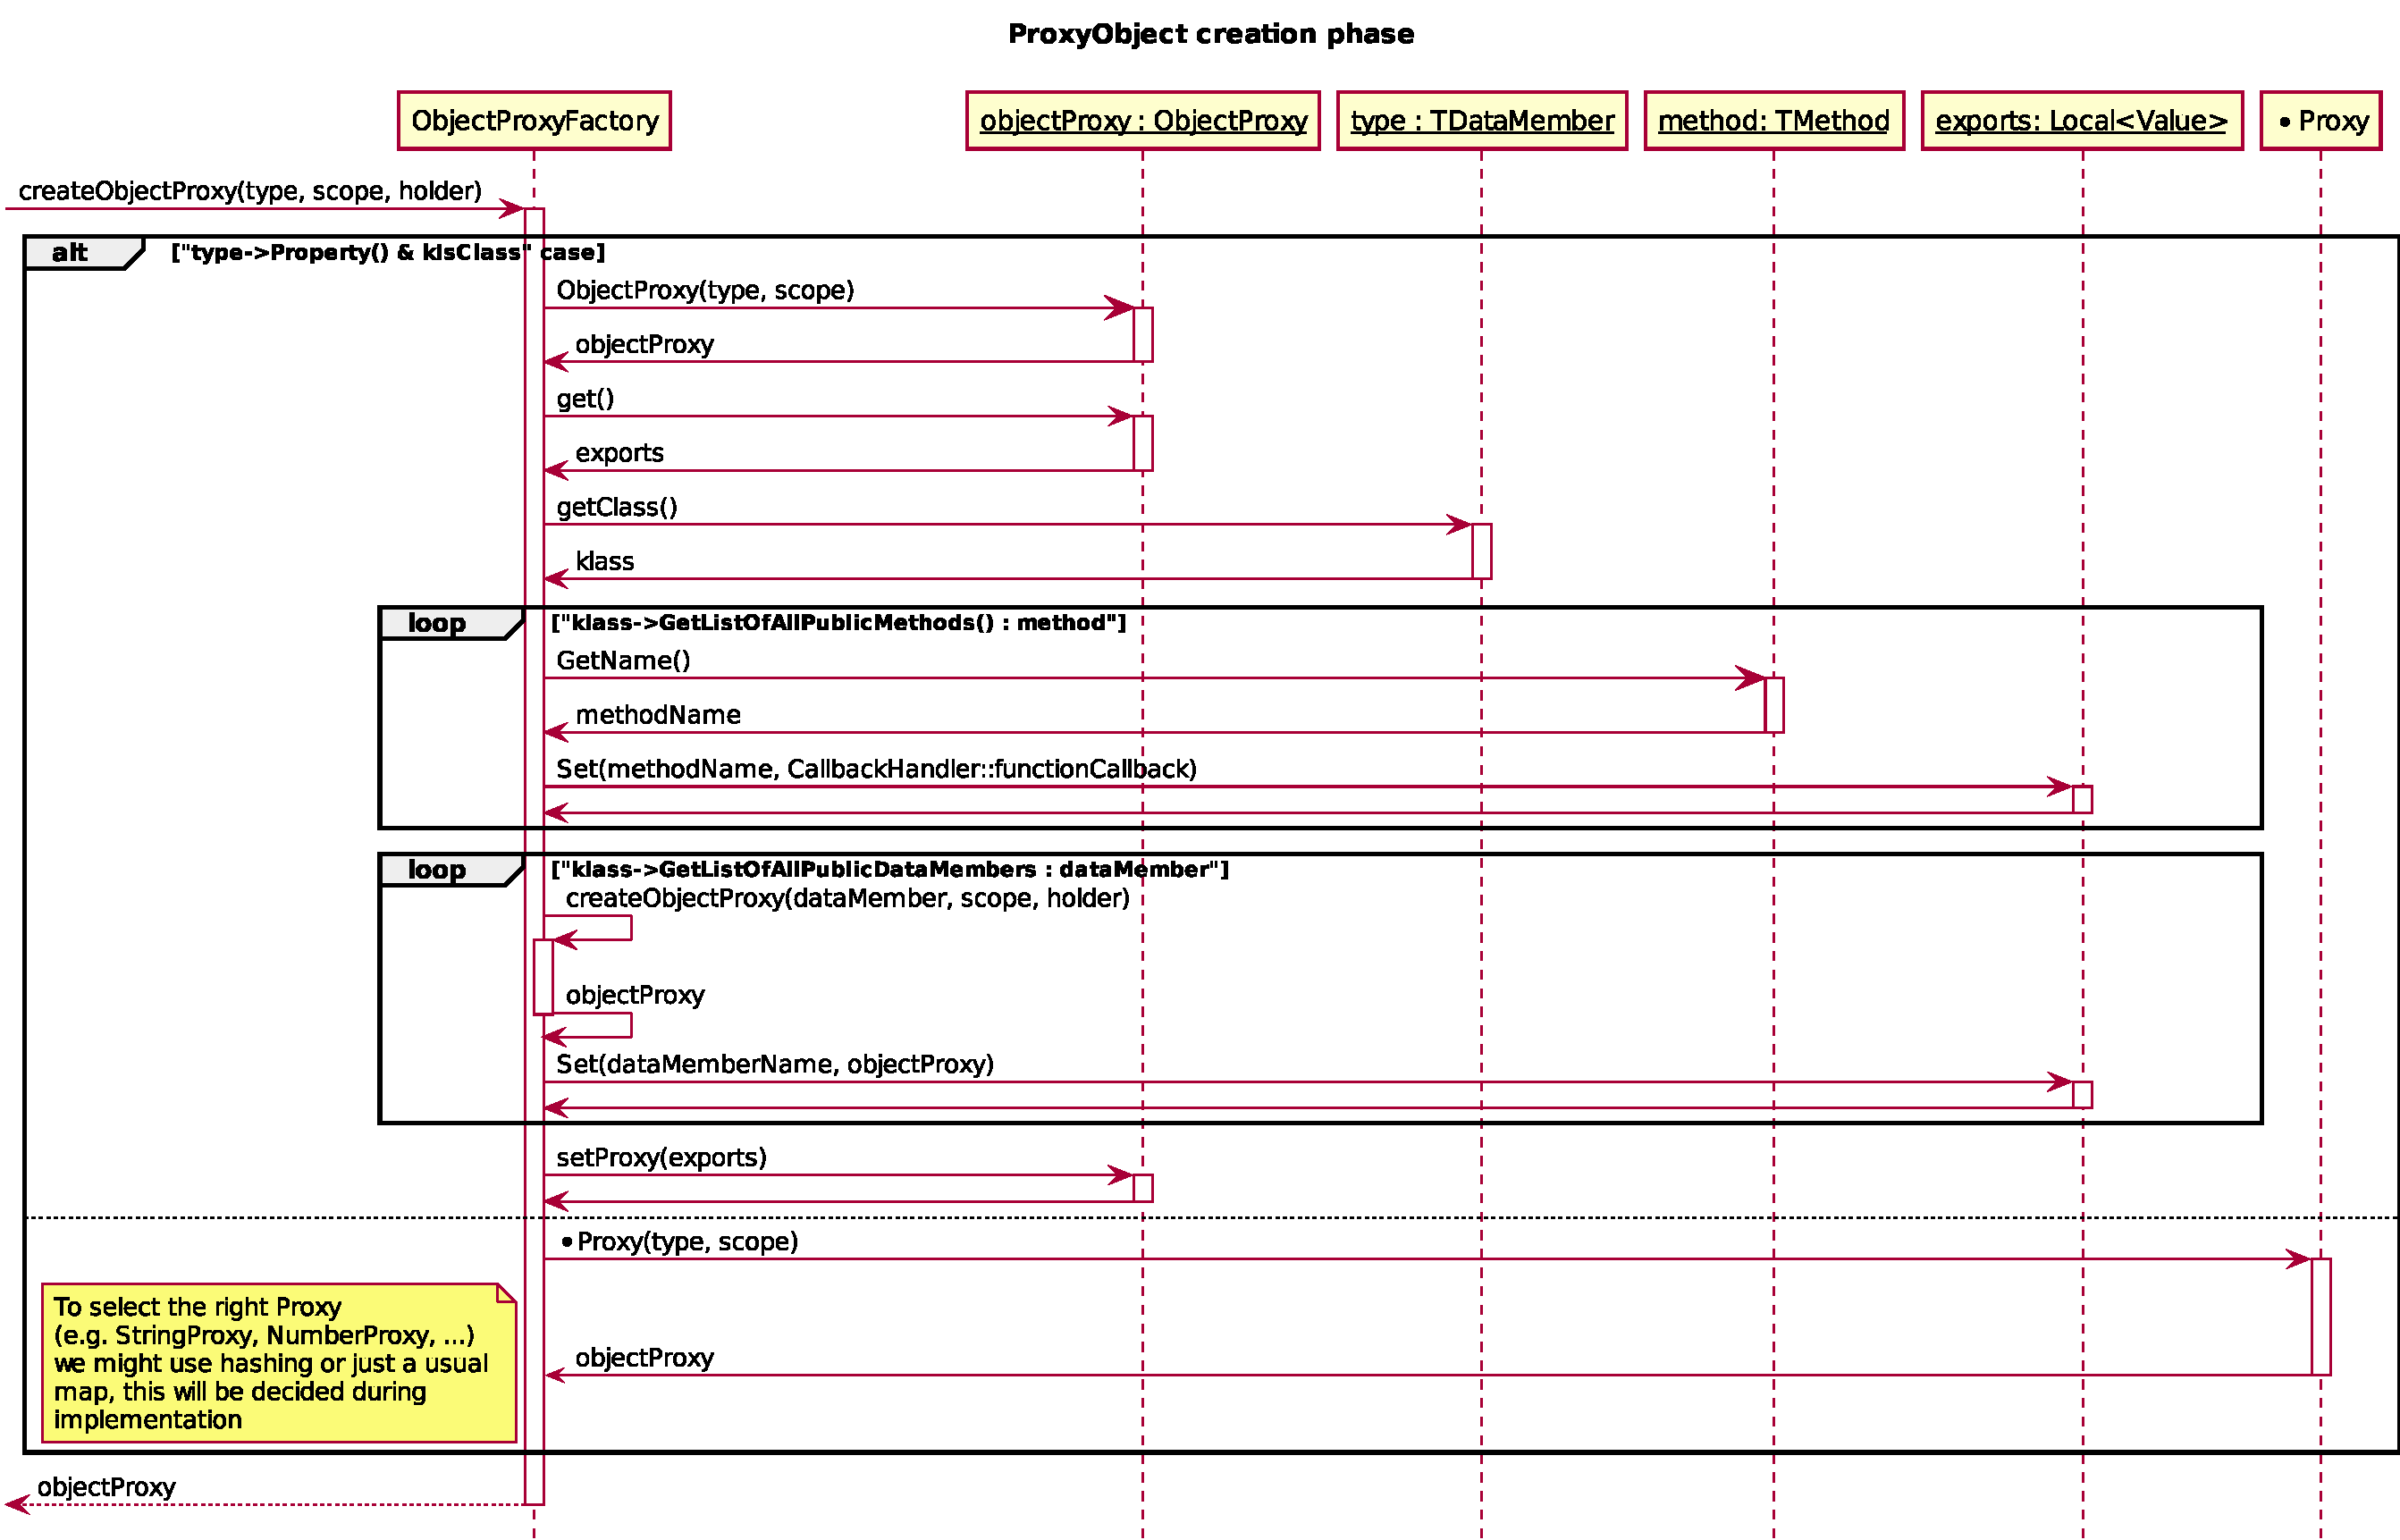
\includegraphics[width=18cm]{./latex/resources/createProxyObject.pdf}
	\caption{object proxy createion sequence}
\end{figure} \pagebreak
\section{createObjectProxy}
\begin{longtable}{p{3cm} @{\hskip 1cm} p{12cm}}
 \hline
\textit{Name} & \texttt{ObjectProxyFactory::createObjectProxy(type: TDataMember, scope: TClassRef, holder: ObjectProxy)}\\
\hline
 \textit{Visibility} & public\\
\hline
\textit{Parameters} & \textit{type: TDataMember} The type identification which the ObjectProxy will have \\
& \textit{scope: TClassRef} The class the ObjectProxy belongs to \\
& \textit{holder: ObjectProxy}  The holder is the ObjectProxy which will encapsulate and hold the newly created ObjectProxy \\
\hline
\textit{Return value} & \textbf{ObjectProxy} Returns the ObjectProxy which is created with the given parameters.\\
  \hline
 \textit{Behavior} & A new ObjectProxy is created each time the createObjectProxy method is called up. \\
\hline
\end{longtable} \pagebreak

\chapter{ObjectProxy}
The \textit{ObjectProxy} class is used to represent ROOT objects. It differentiates between primitive and non-primitive object types.\\
There are the following implementations of \textit{ObjectProxy}:
\begin{itemize}
\item \textbf{EnumProxy} Maps C++ enums to JavaScript strings
\item \textbf{StructProxy} Maps C++ structs to JavaScript objects
\item \textbf{ArrayProxy} Maps C++ arrays to JavaScript arrays, we cannot enlarge C++ arrays, so we will throw an Exception on overflows
\item \textbf{PointerProxy} Maps C++ pointers to JavaScript objects
\item \textbf{NumberProxy} Uses a C++ template to map all C++ numbers to JavaScript Numbers
\item \textbf{StringProxy} Maps C++ strings and c-strings to JavaScript strings
\item \textbf{BooleanProxy} Maps C++ root boolean to Javascript boolean
\end{itemize}
The \textit{ObjectProxyFactory} decides which \textit{ObjectProxy} needs to be instantiated.
Internally all these \textit{ObjectProxies} work the same way by linking a \textit{v8::Local} with a \textit{TDataMember}
\section{ObjectProxy}
\begin{longtable}{p{3cm} @{\hskip 1cm} p{12cm}}
 \hline
\textit{Name} & \texttt{ObjectProxy::ObjectProxy(type: TDataMember, scope: TClassRef)}\\
\hline
 \textit{Visibility} & public\\
\hline
\textit{Parameters} & \textit{type TDataMember} The type of the object \\ & \textit{scope TClassRef} The reference to the class of the object \\
\hline
\textit{Return value} & \textbf{<<constructor>>} the newly constructed ObjectProxy\\
  \hline
  \textit{Behavior} & Creates a new ObjectProxy with the given type and scope.\\
\hline
\end{longtable} \pagebreak
 \section{getType}
\begin{longtable}{p{3cm} @{\hskip 1cm} p{12cm}}
 \hline
\textit{Name} & \texttt{ObjectProxy::getType()}\\
\hline
 \textit{Visibility} & public\\
\hline
\textit{Parameters} & \textit{none}\\
\hline
\textit{Return value} & \textbf{TDataMember} the type of the ObjectProxy\\
  \hline
 \textit{Behavior} & Returns the type of the Object behind the proxy.\\
\hline
\end{longtable} \pagebreak
 \section{set}
\begin{longtable}{p{3cm} @{\hskip 1cm} p{12cm}}
 \hline
\textit{Name} & \texttt{ObjectProxy::set(value: ObjectProxy)}\\
\hline
 \textit{Visibility} & public\\
\hline
\textit{Parameters} & \textit{value: ObjectProxy} the value to set\\
\hline
\textit{Return value} & \textbf{none}\\
  \hline
 \textit{Behavior} & Sets the value of the Object behind the proxy.\\
\hline
\end{longtable} \pagebreak
 \section{get}
\begin{longtable}{p{3cm} @{\hskip 1cm} p{12cm}}
 \hline
\textit{Name} & \texttt{ObjectProxy::get()}\\
\hline
 \textit{Visibility} & public\\
\hline
\textit{Parameters} & \textit{none}\\
\hline
\textit{Return value} & \textbf{Local<Value>} The value the object has.\\
  \hline
 \textit{Behavior} & Returns the value that was set for the object.\\
\hline
\end{longtable} \pagebreak
 \section{setProxy}
\begin{longtable}{p{3cm} @{\hskip 1cm} p{12cm}}
 \hline
\textit{Name} & \texttt{ObjectProxy::setProxy(proxy: Local<Object>)}\\
\hline
 \textit{Visibility} & public\\
\hline
\textit{Parameters} & \textit{proxy: Local<Object>} The v8 object which will be proxy of the ROOT object. \\
\hline
\textit{Return value} & \textbf{none}\\
  \hline
 \textit{Behavior} & Sets \textit{proxy: Local<Object>} to be the proxy of the ROOT object. \\
\hline
\end{longtable} \pagebreak
 \section{getProxy}
\begin{longtable}{p{3cm} @{\hskip 1cm} p{12cm}}
 \hline
\textit{Name} & \texttt{ObjectProxy::getProxy()}\\
\hline
 \textit{Visibility} & public\\
\hline
\textit{Parameters} & \textit{none}\\
\hline
\textit{Return value} & \textbf{Local<Object>} The current proxy of the ROOT object. \\
  \hline
 \textit{Behavior} & Gets the proxy of the ROOT object. \\
\hline
\end{longtable} \pagebreak
 \section{isPrimitive}
\begin{longtable}{p{3cm} @{\hskip 1cm} p{12cm}}
 \hline
\textit{Name} & \texttt{ObjectProxy::isPrimitive()}\\
\hline
 \textit{Visibility} & public\\
\hline
\textit{Parameters} & \textit{none}\\
\hline
\textit{Return value} & \textbf{bool} Whether or not the represented object is of a primitive type or not.\\
  \hline
  \textit{Behavior} & Returns \textit{true} if the represented object's type is primitive, \textit{false} if not.\\
\hline
\end{longtable} \pagebreak


\chapter{Appendix}
\section{Class diagram} % Object Model

\begin{figure}[htb]
	\centering
	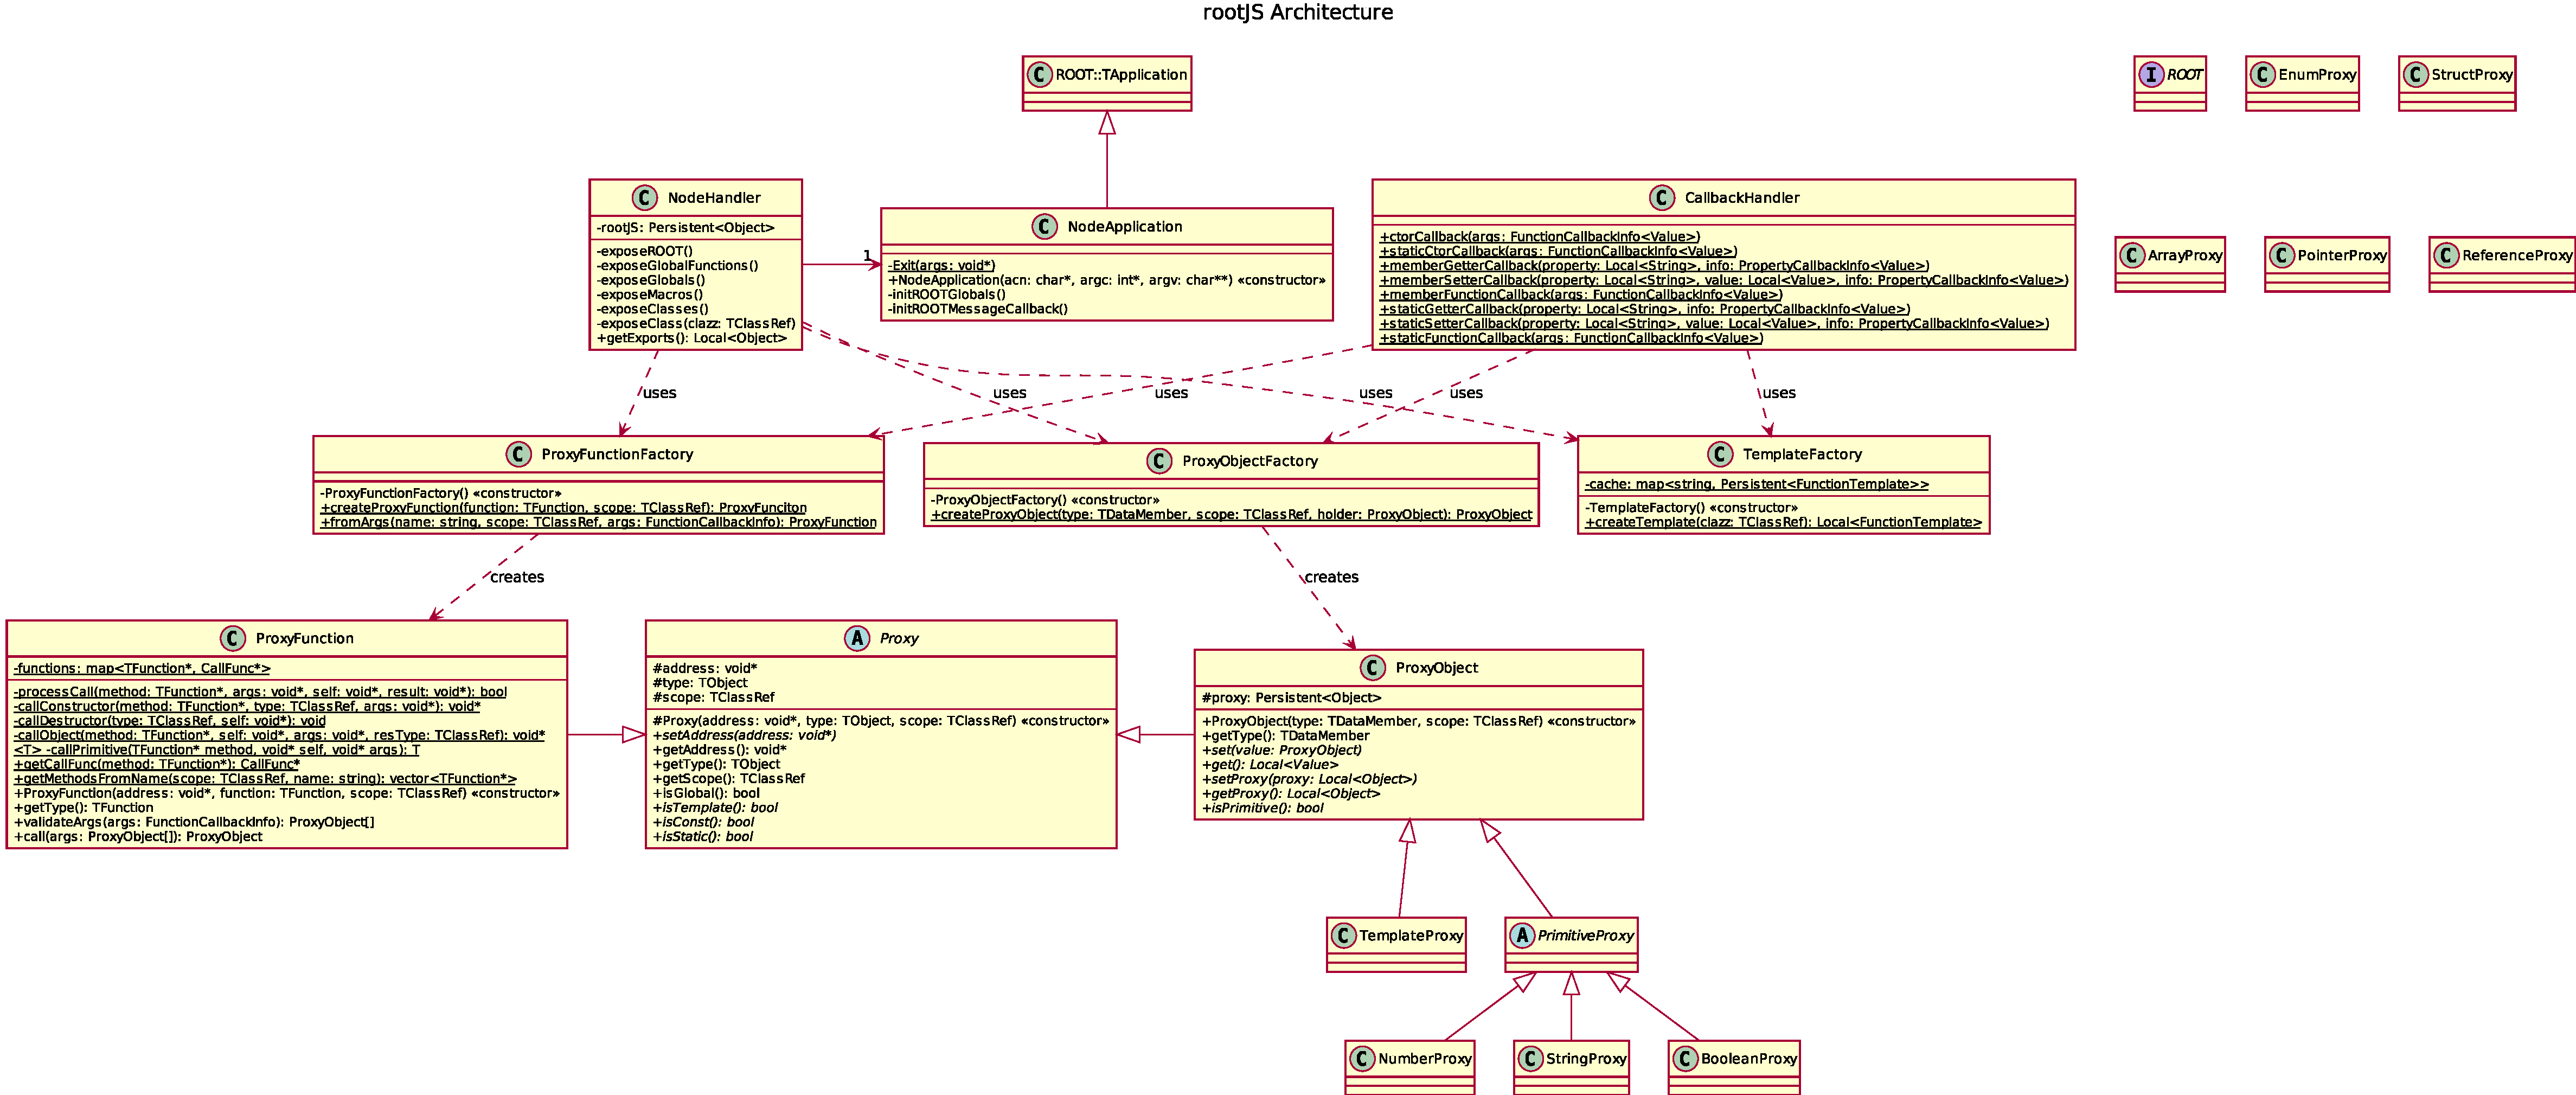
\includegraphics[width=\textheight, height=\linewidth, angle={90}, keepaspectratio]{./latex/resources/architecture.pdf}
	\caption{rootJS class diagram}
\end{figure}

\pagebreak

\section{Dynamic Model}

\begin{figure}[htb]
	\centering
	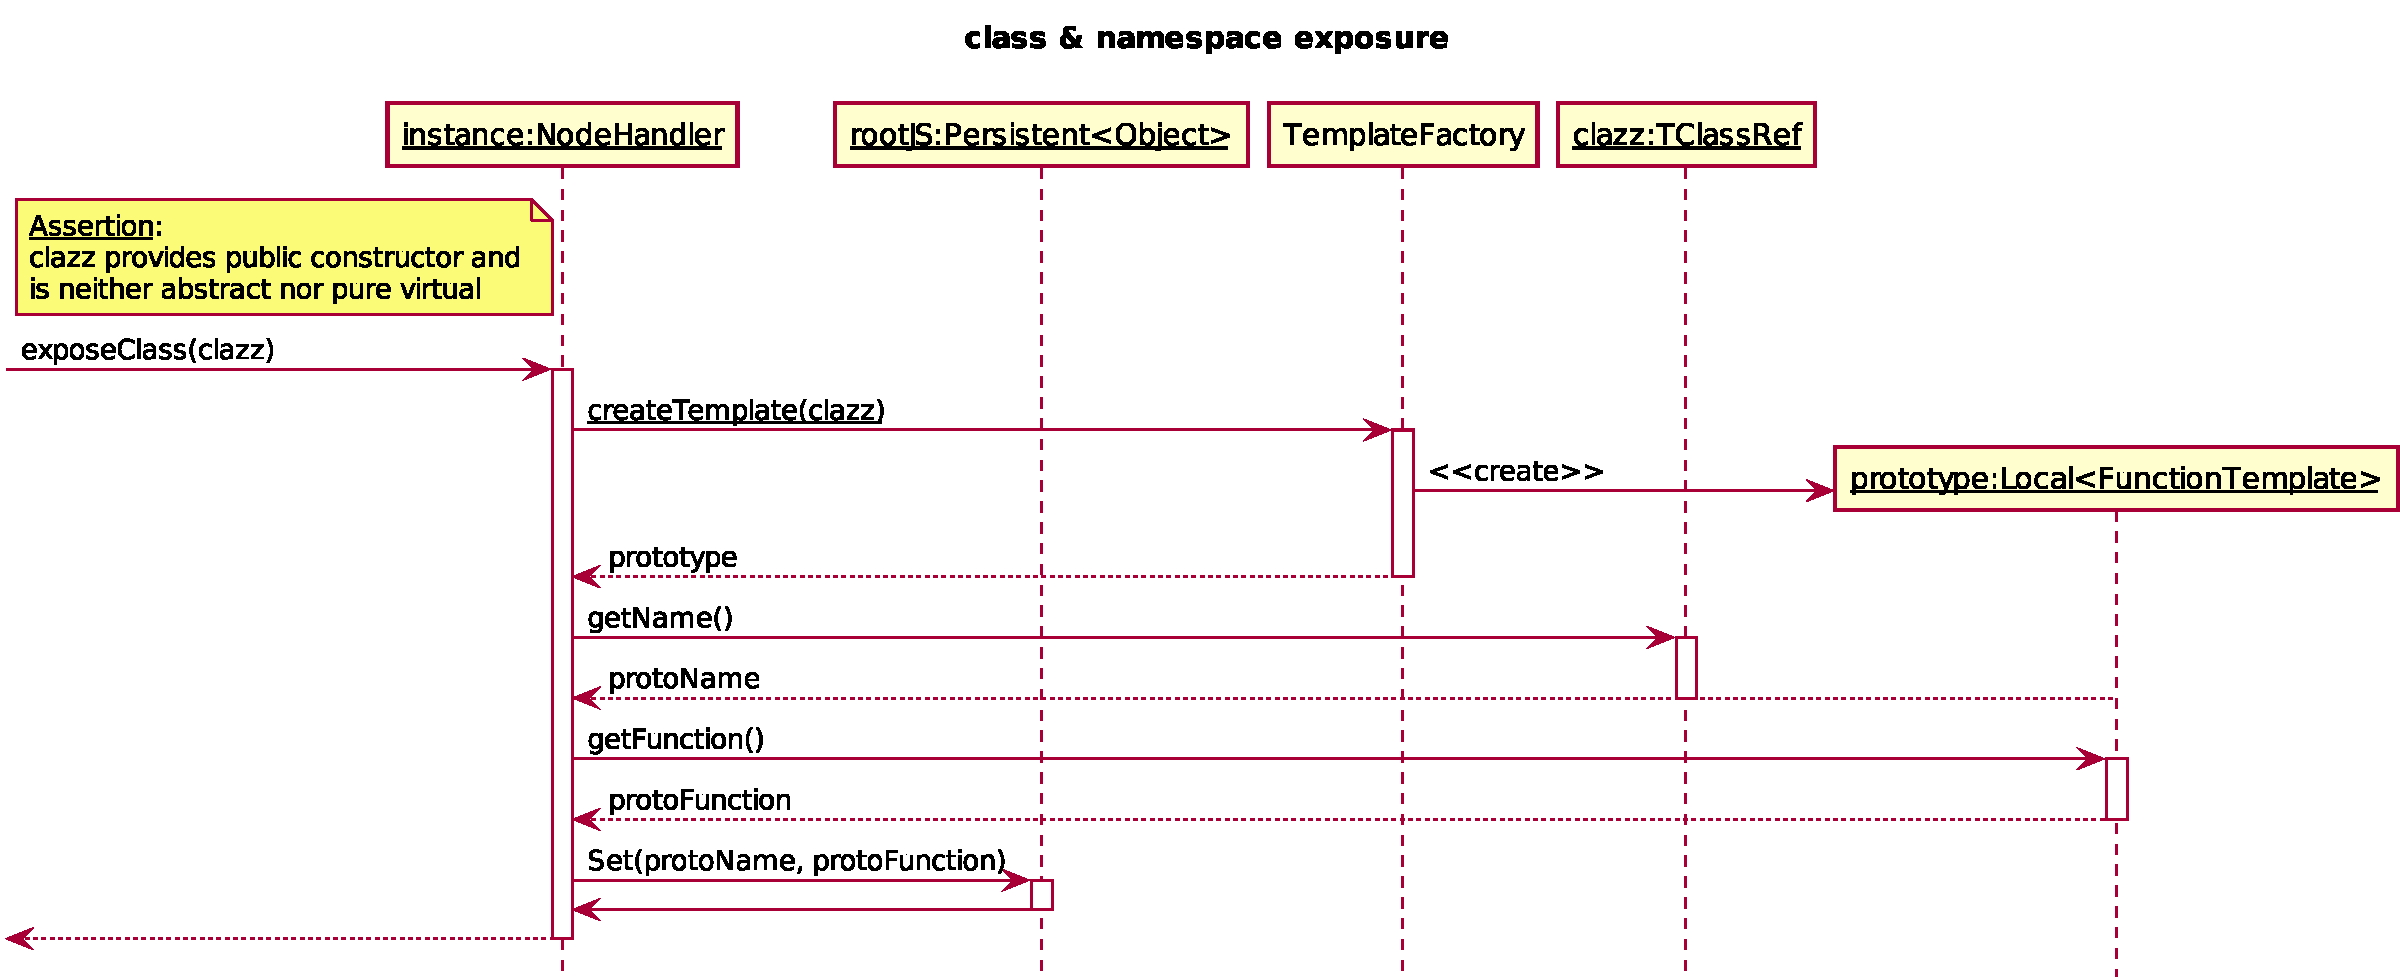
\includegraphics[width=18cm]{./latex/resources/classExposureSequence.pdf}
	\caption{class exposure sequence}
\end{figure}

\begin{figure}[htb]
	\centering
	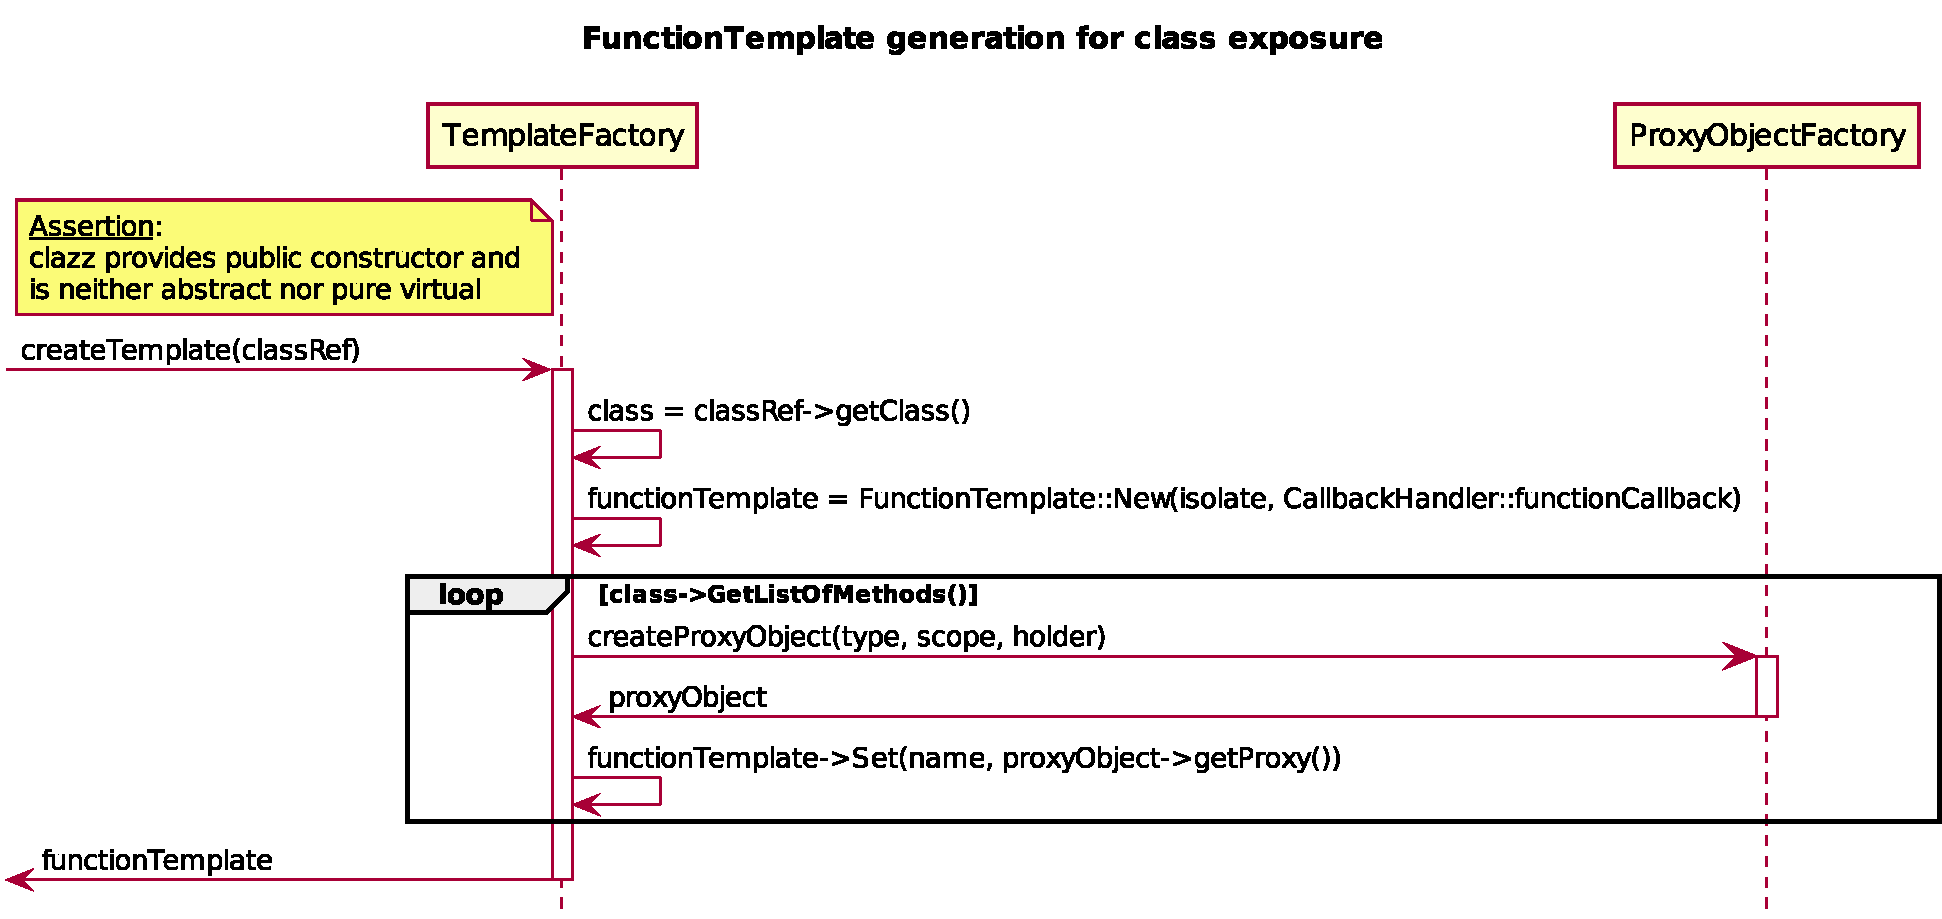
\includegraphics[width=18cm]{./latex/resources/functionTemplateGenerate.pdf}
	\caption{class exposure sequence}
\end{figure}

\begin{figure}[htb]
	\centering
	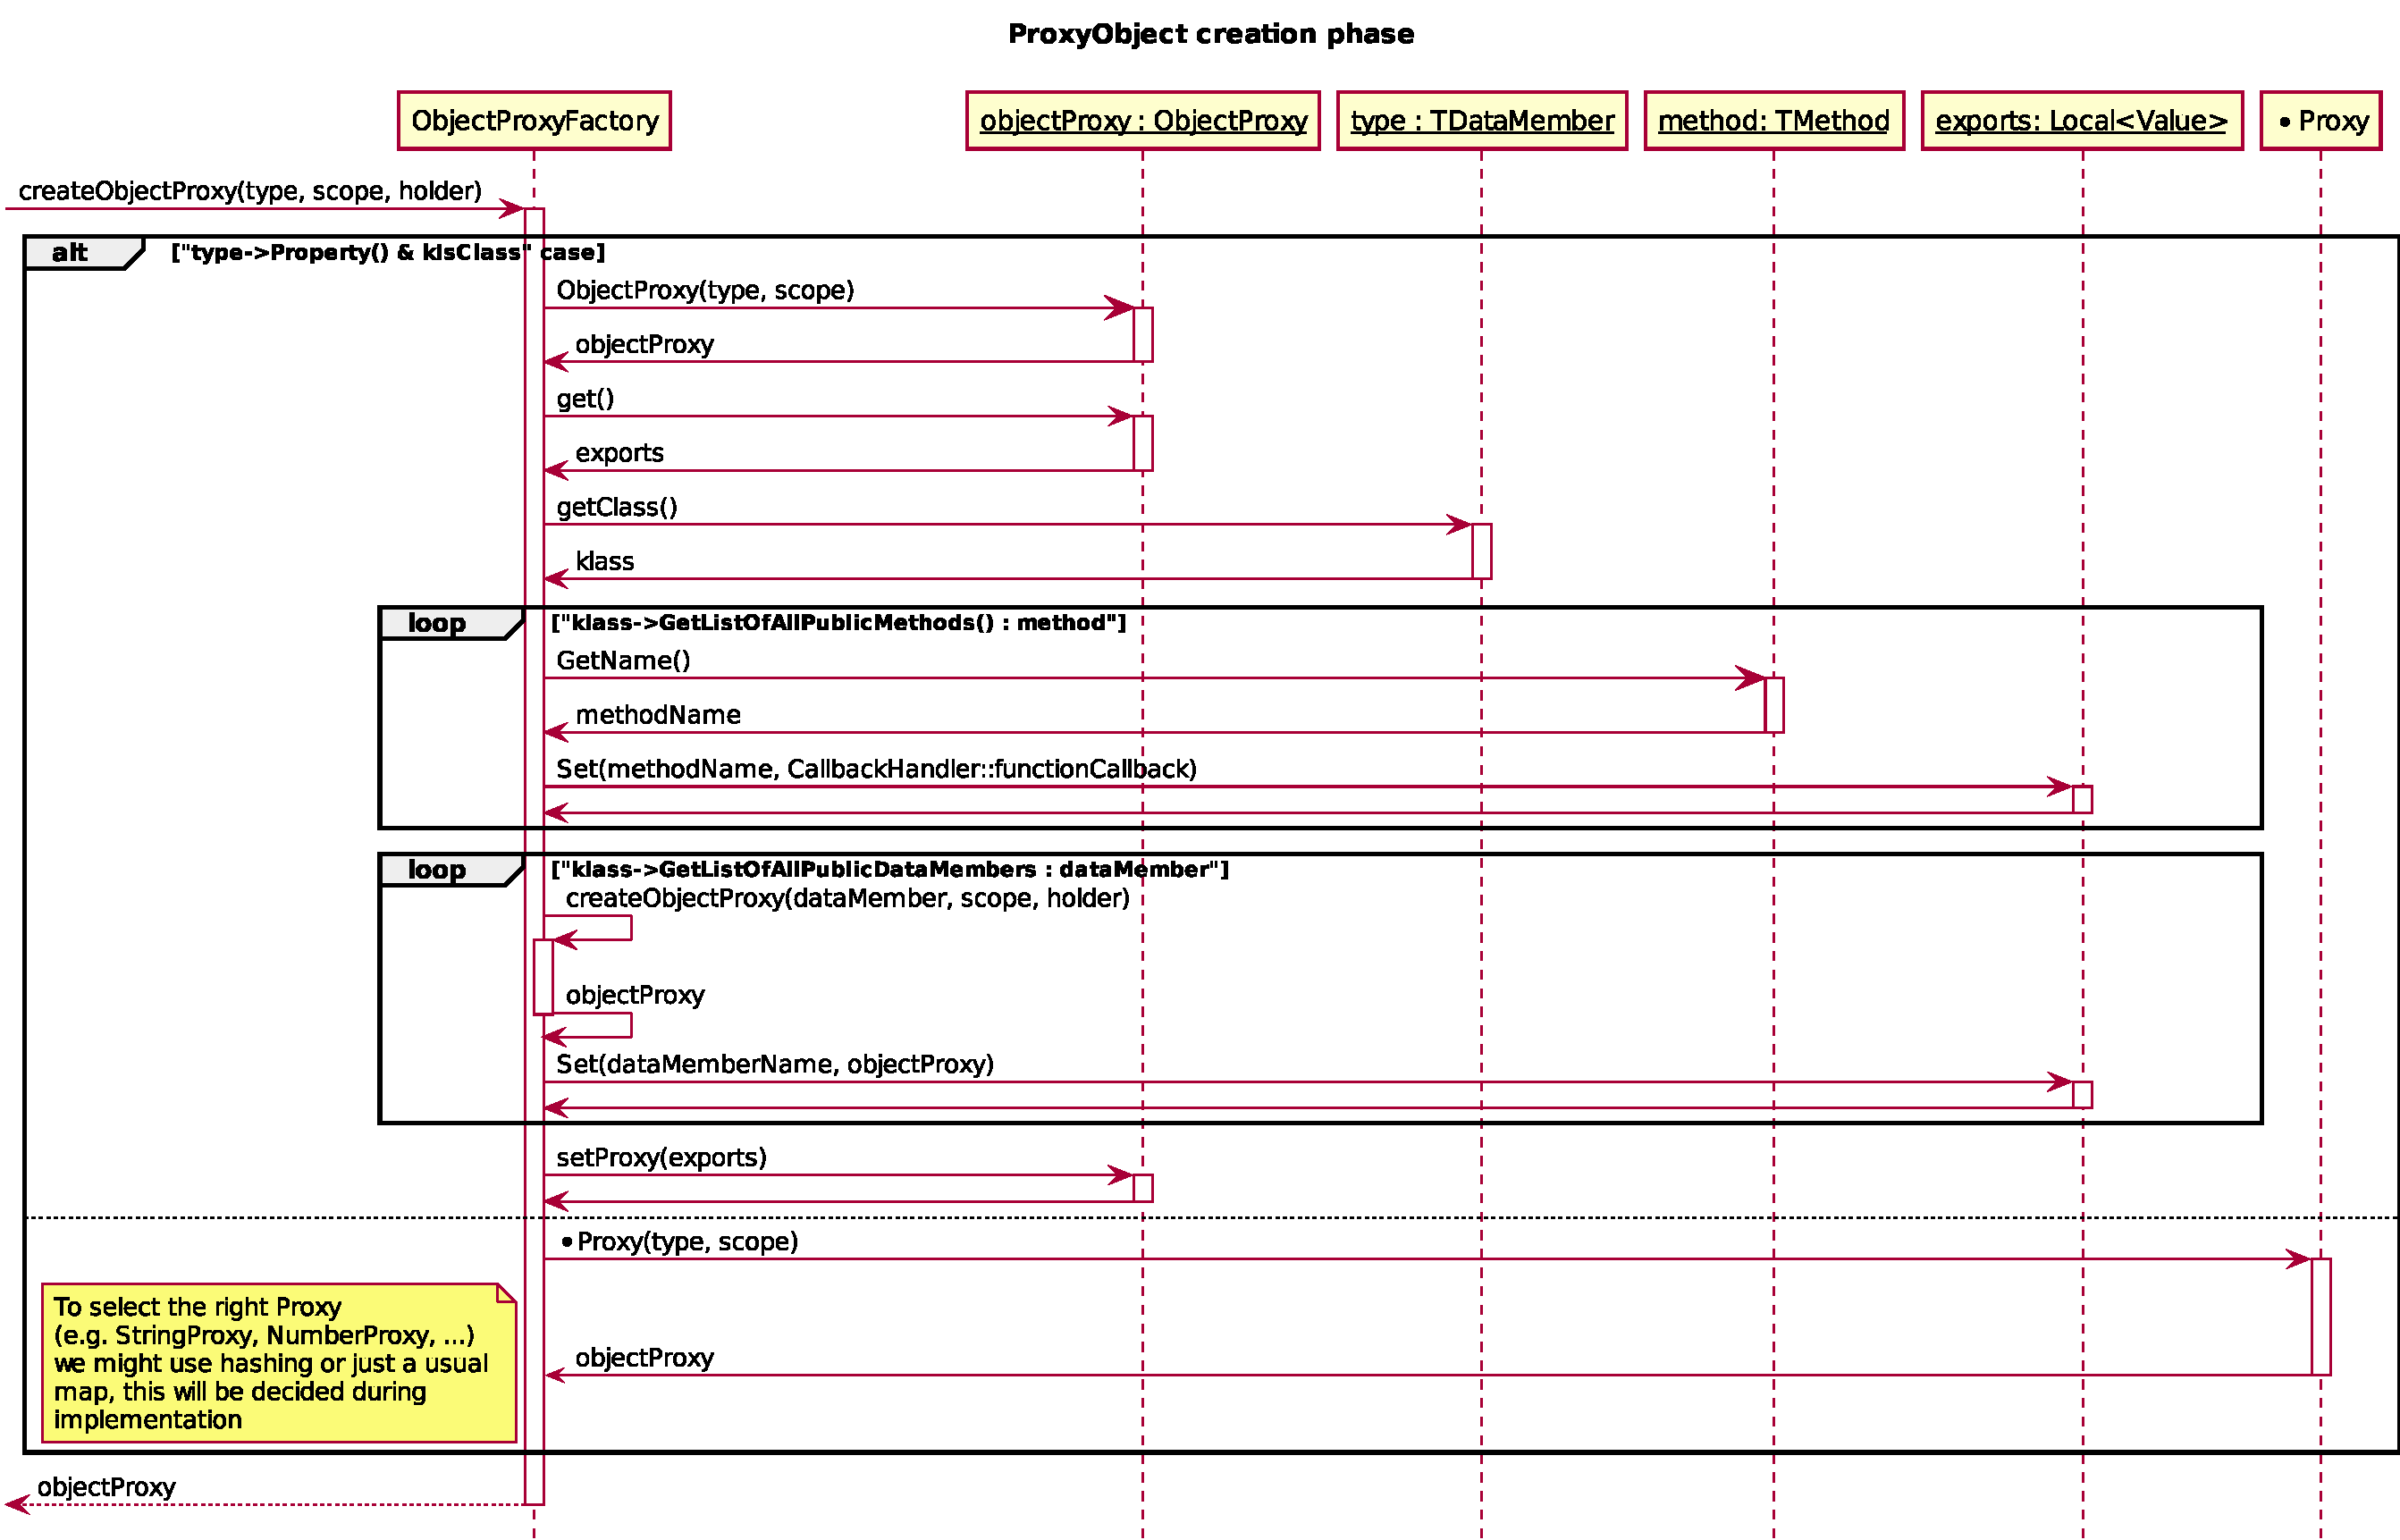
\includegraphics[width=18cm]{./latex/resources/createProxyObject.pdf}
	\caption{ProxyObject creation sequence}
\end{figure}

\newpage

\section{Glossary}
\paragraph{Callback}
A function which is passed as an argument to some code, which is then expected to call the argument back.
\paragraph{Constructor}
A method which is used to create an object.
\paragraph{Encapsulation}
A piece of functionality of certain languages used to restrict access to some of the object's variables and methods
\paragraph{Instance}
A created object.
\paragraph{Proxy}
A class functioning as an intermediary between two classes.
\paragraph{Static}
A method which does not require the object to be instantiated.
\paragraph{Template} 
A feature of C++ that allows classes and functions to operate with generic types.
\paragraph{v8} 
An open source JavaScript engine, written in C++ and made by Google.

\newpage




\end{document}
